\documentclass[aspectratio=169,11pt]{beamer}
\usepackage[T1]{fontenc}
\usepackage{lmodern}
\usepackage{booktabs}
\usepackage{array}
\usepackage{ragged2e}
\usepackage{tikz}
\usetikzlibrary{arrows.meta,positioning,shapes.geometric}
\usepackage{xcolor}
\usepackage{amsmath}

\definecolor{NITNavy}{RGB}{18,42,76}
\definecolor{NITBlue}{RGB}{39,91,145}
\definecolor{NITLight}{RGB}{232,241,250}
\definecolor{NITGray}{RGB}{95,95,95}

\setbeamercolor{normal text}{fg=black,bg=white}
\setbeamercolor{frametitle}{fg=NITNavy}
\setbeamercolor{structure}{fg=NITBlue}
\setbeamercolor{title}{fg=NITNavy}
\setbeamertemplate{navigation symbols}{}
\setbeamertemplate{footline}{\hfill\insertframenumber\hspace{0.5cm}\vspace{0.15cm}}
\setbeamertemplate{frametitle}{
  \vspace{0.18cm}\begin{beamercolorbox}[wd=\paperwidth,sep=0.12cm,leftskip=0.55cm]{frametitle}
  \insertframetitle
  \end{beamercolorbox}
  \vspace{-0.05cm}\hspace{0.55cm}\rule{0.91\paperwidth}{0.6pt}
}

\newcommand{\NITHeader}{
\begin{center}
{\large\bfseries National Institute of Technology Tiruchirappalli}\\[-1mm]
{\normalsize\bfseries Department of Computer Science and Engineering}
\end{center}
\vspace{-2mm}\hrule\vspace{3mm}
}

\title{Evolutionary and Generative AI Approaches\\for Fraud Detection in Healthcare Insurance Claims}
\author{Thirilokkiyan K\\Roll No.: 206125028\\Guide: Dr. C. Mala}
\institute{M.Tech Project Work -- Phase 1}
\date{}

\begin{document}

\begin{frame}
\NITHeader
\titlepage
\end{frame}

\begin{frame}{Introduction -- Part 1}
\begin{itemize}
\item Healthcare fraud is a major global problem: fraudulent claims drain billions of dollars and divert resources away from genuine patients.
\item Examples: the U.S. Justice Department charged nearly 200 individuals in a \$2.7 billion healthcare-fraud crackdown (2024); Medicare scams alone have resulted in over \$100 million in fake claims.
\item China's healthcare spending reached RMB 23 trillion in 2021, with $\sim$10\% lost to false claims; the U.S. loses an estimated USD 120--410 billion annually to healthcare fraud.
\item Traditional rule-based and manual detection methods struggle as fraud schemes become more sophisticated and adaptive.
\end{itemize}
\end{frame}

\begin{frame}{Introduction -- Part 2}
\begin{columns}[T]
\column{0.48\textwidth}
\begin{block}{Challenge 1: High Dimensionality}
Claims contain dozens to hundreds of patient, provider, policy and billing features.
\end{block}
\column{0.48\textwidth}
\begin{block}{Challenge 2: Severe Class Imbalance}
Fraudulent claims are rare (often $<10\%$), biasing models toward legitimate claims.
\end{block}
\end{columns}
\vspace{3mm}
\begin{itemize}
\item Machine learning and evolutionary/generative AI techniques offer promising solutions.
\item Metaheuristic optimization: WOA and GA for parameter tuning and feature selection.
\item Generative models: GANs and LLM-based synthesis to address data scarcity and imbalance.
\item This project reviews and builds upon \textbf{DW-WOA-SVM} and \textbf{WCGAN-GA-RF}.
\end{itemize}
\end{frame}

\begin{frame}{Literature Survey -- Existing Solutions}
\scriptsize
\begin{tabular}{p{0.05\textwidth}p{0.31\textwidth}p{0.25\textwidth}p{0.31\textwidth}}
\toprule
\textbf{S.No.} & \textbf{Paper Details} & \textbf{Techniques Used} & \textbf{Gaps Identified}\\
\midrule
1 & Nabrawi \& Alanazi, ``Fraud detection in healthcare insurance claims using machine learning,'' \emph{Risks}, 2023 &
Random Forest; Logistic Regression; ANN &
No handling of high dimensionality; limited optimization-based tuning.\\
2 & Tubishat et al., ``Leveraging evolutionary algorithms with a dynamic weighted search space approach for fraud detection in healthcare insurance claims,'' \emph{Knowledge-Based Systems}, 2025 &
DW-WOA-SVM; dynamic search space; feature weighting; LLM synthetic data &
Nested cross-validation is computationally expensive; synthetic data may not reflect real-world fraud diversity; extensive testing focused on WOA-family methods.\\
3 & Cai et al., ``WCGAN-GA-RF: Healthcare Fraud Detection via Generative Adversarial Networks and Evolutionary Feature Selection,'' \emph{Information}, 2026 &
WCGAN-GP; GA feature selection; Random Forest &
Precision--recall trade-off; single China regional dataset; GAN training cost $\sim$15 min/run on GPU.\\
\bottomrule
\end{tabular}
\end{frame}

\begin{frame}{Literature Survey -- Existing Solutions}
\scriptsize
\begin{tabular}{p{0.05\textwidth}p{0.31\textwidth}p{0.25\textwidth}p{0.31\textwidth}}
\toprule
\textbf{S.No.} & \textbf{Paper Details} & \textbf{Techniques Used} & \textbf{Gaps Identified}\\
\midrule
4 & Sowah et al., ``Decision support system (DSS) for fraud detection in health insurance claims using genetic support vector machines (GSVMs),'' \emph{J. Eng.}, 2019 &
Genetic Algorithm + SVM &
Limited to Ghana National Health Insurance dataset; no dynamic search space or feature weighting.\\
5 & Majhi et al., ``Fuzzy clustering algorithm based on modified whale optimization algorithm for automobile insurance fraud detection,'' \emph{Evol. Intell.}, 2021 &
Modified WOA + Fuzzy C-Means &
Automobile insurance rather than healthcare; clustering-based rather than directly optimized classification.\\
6 & Mao et al., ``XGAN: A medical insurance fraud detector based on GAN with XGBoost,'' \emph{J. Inf. Hiding Mult. Signal Process.}, 2024 &
GAN oversampling + XGBoost &
Mode collapse/training instability risk; no feature-selection component.\\
\bottomrule
\end{tabular}
\end{frame}

\begin{frame}{Literature Survey -- Summary \& Transition}
\begin{block}{Gap 1}
Data scarcity/imbalance is addressed inconsistently; simple SMOTE/ADASYN may be limited for high-dimensional sparse data.
\end{block}
\begin{block}{Gap 2}
Feature selection and parameter tuning are often treated separately rather than jointly optimized.
\end{block}
\begin{itemize}
\item DW-WOA-SVM addresses optimization through a dynamic weighted search space and WOA-based tuning.
\item WCGAN-GA-RF addresses imbalance through generative augmentation and feature selection through GA.
\item \textbf{Project direction:} combine the complementary insights of optimization, augmentation, feature selection and classification.
\end{itemize}
\end{frame}

\begin{frame}{Motivation \& Problem Statement}
\begin{columns}[T]
\column{0.48\textwidth}
\begin{block}{Motivation}
\begin{itemize}
\item Fraud detection directly impacts financial integrity and patient-care quality.
\item Existing solutions often tackle either optimization or data imbalance, but rarely combine both effectively.
\item High-quality, richly-featured real-world datasets are limited.
\end{itemize}
\end{block}
\column{0.48\textwidth}
\begin{block}{Problem Statement}
\begin{itemize}
\item Poor generalization arises from severe class imbalance and high-dimensional, noisy feature spaces.
\item An integrated framework is needed to combine synthetic generation, feature selection and optimized classification.
\item The framework should improve detection accuracy while maintaining interpretability and computational feasibility.
\end{itemize}
\end{block}
\end{columns}
\end{frame}

\begin{frame}{Objectives}
\begin{enumerate}
\item Study and compare evolutionary (WOA-based) and generative (GAN-based) approaches for healthcare fraud detection.
\item Design/evaluate a pipeline combining synthetic data augmentation, feature weighting/selection and classifier parameter optimization.
\item Evaluate Accuracy, Precision, Recall and F1-score against baseline classifiers and SMOTE/ADASYN/ROS.
\item Analyze feature importance for interpretability, including claim frequency, provider consistency and billing patterns.
\item Assess computational efficiency and scalability for potential real-world deployment.
\end{enumerate}
\end{frame}

\begin{frame}{Block Schematic / Modular Diagram}
\centering
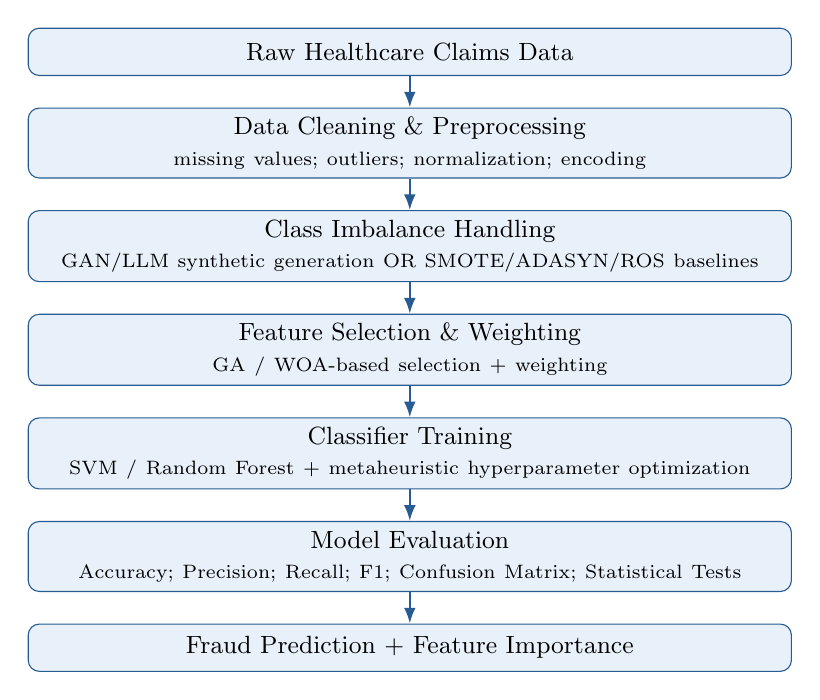
\begin{tikzpicture}[node distance=4mm,
box/.style={rectangle,rounded corners,draw=NITBlue,fill=NITLight,align=center,text width=0.78\textwidth,minimum height=6mm,font=\small},
arrow/.style={-{Latex[length=2mm]},draw=NITBlue,thick}]
\node[box] (a) {Raw Healthcare Claims Data};
\node[box,below=of a] (b) {Data Cleaning \& Preprocessing\\\scriptsize missing values; outliers; normalization; encoding};
\node[box,below=of b] (c) {Class Imbalance Handling\\\scriptsize GAN/LLM synthetic generation OR SMOTE/ADASYN/ROS baselines};
\node[box,below=of c] (d) {Feature Selection \& Weighting\\\scriptsize GA / WOA-based selection + weighting};
\node[box,below=of d] (e) {Classifier Training\\\scriptsize SVM / Random Forest + metaheuristic hyperparameter optimization};
\node[box,below=of e] (f) {Model Evaluation\\\scriptsize Accuracy; Precision; Recall; F1; Confusion Matrix; Statistical Tests};
\node[box,below=of f] (g) {Fraud Prediction + Feature Importance};
\foreach \x/\y in {a/b,b/c,c/d,d/e,e/f,f/g}{\draw[arrow] (\x)--(\y);}
\end{tikzpicture}
\end{frame}

\begin{frame}{Expected Milestones / Work Plan}
\begin{enumerate}
\item \textbf{Literature Survey:} finalize review of DW-WOA-SVM, WCGAN-GA-RF and related methods.
\item \textbf{Dataset \& Preprocessing:} prepare claims data; clean, encode, normalize and analyze imbalance.
\item \textbf{Baseline Models:} implement SVM, Random Forest and SMOTE/ADASYN/ROS baselines.
\item \textbf{Proposed Pipeline:} integrate synthetic augmentation, GA/WOA feature selection and classifier optimization.
\item \textbf{Evaluation \& Analysis:} compare Accuracy, Precision, Recall, F1, confusion matrices and computational cost.
\item \textbf{Interpretability \& Reporting:} analyze feature importance and consolidate results, limitations and future work.
\end{enumerate}
\vspace{2mm}
{\scriptsize\textit{Note: the supplied content specified the work-plan heading but did not provide milestone dates; the above is a proposed sequence for the project.}}
\end{frame}

\end{document}
